\section{Models with more than one channel type}
Now the original Morris-Lecar model is considered, where there is a three-dimensional phase space.
In the original treatment of voltage oscillations  in barnacle muscle fibres the calcium gating variable $m$ is included as a dynamical variable, sot the total system is describes with the following deterministic equations:

\begin{align*}
	\frac{dv}{dt} = F(v, n, m) =&\frac{1}{C}(I_{app}-g_L(v-v_L)+\\
															&-g_{Ca}m(v-v_Ca)-g_Kn(v-v_K))
\end{align*}

\begin{align*}
	\frac{dn}{dt} &= G(v, n, m) = \alpha_n(v)(1-n)-\beta_n(v)n=\\
								&=\frac{n_{\infty}(v)-n}{\tau_n(v)}
\end{align*}

\begin{align*}
	\frac{dm}{dt} &= H(v, n, m) = \alpha_m(v)(1-m)-\beta_m(v)m=\\
								&=\frac{m_\infty(v)-m}{\tau_m(v)}
\end{align*}

The number of calcium gates evolves according to this equation instead of being set to its asymptotic value $m_\infty = \frac{\alpha_m}{\alpha_m+\beta_m}$.
The planar form of the equation is obtained by observing that $m$ approaches equilibrium faster than $n$ and $v$, so using standard arguments from singular perturbation theory this system can be brought into the planar model by replacing $F$ and $G$ with: $f(v, n) = F(v, n, m_\infty(v))$ and $g(v, n) = G(v, n, m_\infty(v))$.
Now for the $3D$ model $\epsilon_m = \frac{v-v_a}{v_b}$ has to be introduced in addition to $\epsilon_n = \frac{v-v_c}{v_d}$.
It can be noted how $\epsilon_x$ represents where the voltage falls along the activation curve for channel type $x$, relative to its half-activation point ($v_a$ for calcium and $v_c$ for potassium )and its slope (reciprocals of $v_b$ for calcium and $v_d$ for potassium).
The per capita opening and closing rates for each channel type are then:

$$\alpha_m(v) = \frac{\phi_m\cosh\frac{\epsilon_m}{2}}{1+e^{2\epsilon_m}}\quad\beta_m(v) = \frac{\phi_m\cosh\frac{\epsilon_m}{2}}{1+e^{-2\epsilon_m}}$$

$$\alpha_n(v) = \frac{\phi_n\cosh\frac{\epsilon_n}{2}}{1+e^{2\epsilon_n}}\quad\beta_n(v) = \frac{\phi_n\cosh\frac{\epsilon_n}{2}}{1+e^{-2\epsilon_n}}$$

With parameters:

\begin{multicols}{3}
	\begin{itemize}
		\item $v_a = -1.2$.
		\item $v_b = 18$.
		\item $v_c = 2$.
		\item $v_d = 30$.
		\item $\phi_m = 0.4$.
		\item $\phi_n = 0.04$
	\end{itemize}
\end{multicols}

The asymptotic open probabilities are given by $m_\infty$ and $n_\infty$ and the time constants $\tau_m$ and $\tau_n$, which satisfy the relations:

$$m_\infty(v) = \frac{\alpha_m(v)}{\alpha_m(v) + \beta_m(v)} = \frac{1+\tanh\epsilon_m}{2}$$

$$n_\infty(v) = \frac{\alpha_n(v)}{\alpha_n(v) + \beta_n(v)} = \frac{1+\tanh\epsilon_n}{2}$$

$$\tau_m(v) = \frac{1}{\phi\cosh\frac{\epsilon_m}{2}}$$

$$\tau_n(v) = \frac{1}{\phi\cosh\frac{\epsilon_n}{2}}$$

Assuming a population of $M_{tot}$ calcium and $N_{tot}$ potassium gates a stochastic hybrid system is obtained, with a continuous variable $V(t)$ and two discrete ones $M(t)$ and $N(t)$.
The voltage evolves according to the sum of the applied, leak, calcium and potassium currents

\begin{align*}
	\frac{dV}{dt} &=&  F(V(t), N(t), M(t)) = \\
								&=& \frac{1}{C}\biggl(I_{app} - g_L(V(t)-v_L)-g_{Ca}\frac{M(t)}{M_{tot}}(V(t)-v_{Ca}) +\\
								& &- g_K\frac{N(t)}{N_{tot}}(V(t)-v_K)\biggr)
\end{align*}

The number of open gates change only by unit increases and decreases remaining constant between such changes.
So the channel states evolve according to:

\begin{align*}
	M(t) =&M(0) - Y_{close}^M\biggl(\int_0^t\beta_m(V(s))M(s)ds\biggr)+\\
				&+Y_{open}^M\biggl(\int_0^t\alpha_m(V(s))(M_{tot}-M(s))ds\biggr)
\end{align*}

\begin{align*}
	N(t) =&N(0) - Y_{close}^N\biggl(\int_0^t\beta_n(V(s))N(s)ds\biggr)+\\
				&+Y_{open}^N\biggl(\int_0^t\alpha_n(V(s))(N_{tot}-N(s))ds\biggr)
\end{align*}

	\subsection{Deterministic representation}
	Firstly we analysed the trajectory of the fully deterministic model, which can be seen in figure \ref{fig:morris-lecar-4}.

	\begin{figure}
		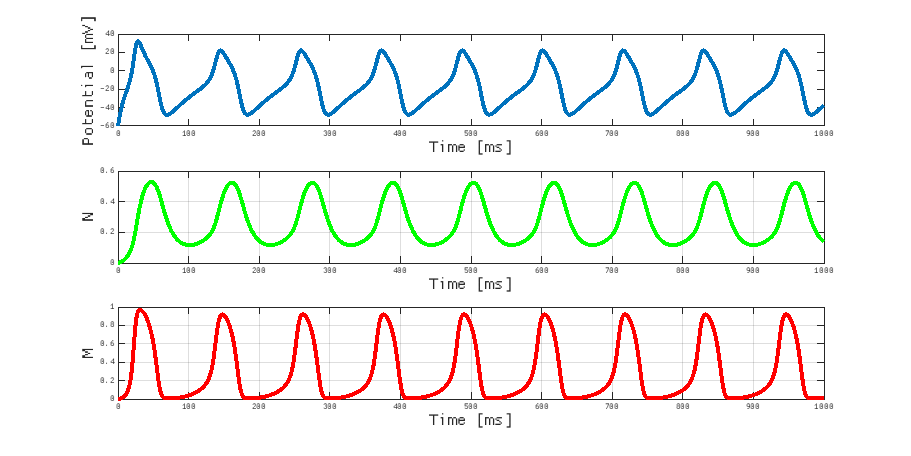
\includegraphics[width=\textwidth]{Figures/morris-lecar-4}
		\caption{Deterministic Morris Lecar model with evolving potassium and calcium dynamics. From top to bottom: \textbf{1} Membrane voltage. \textbf{2} Fraction of open potassium channels. \textbf{3} Fraction of open calcium channels.}
		\label{fig:morris-lecar-4}
	\end{figure}

	\subsection{Random time change representation}
	We simulated the stochastic Morris Lecar model  through the random time change representation for $4000$ seconds.
		The relationship within voltage and the number of open channel can be seen in figure \ref{fig:ml-rtc-4}.

		\begin{figure}
			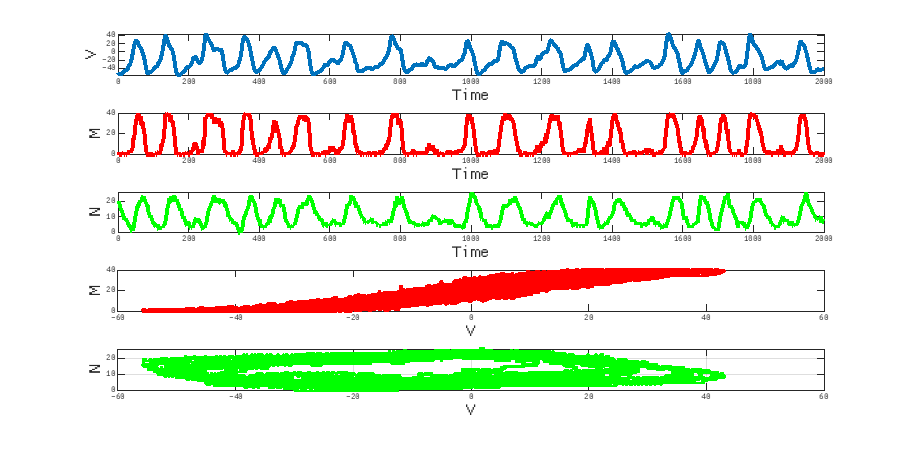
\includegraphics[width=\textwidth]{Figures/ml-rtc-4}
			\caption{The Morris Lecar stochastic model with only potassium channels. From top to bottom: \textbf{1} The membrane voltage. \textbf{2} The number of open calcium channel over time. \textbf{3} The number of open potassium channels over time. \textbf{4} The number of open calcium channel over voltage. \textbf{5} The number of open potassium channel over voltage}
			\label{fig:ml-rtc-4}
		\end{figure}

	\subsection{Gillespie's representation}
	We simulated the stochastic Morris Lecar model through Gillespie's representation for $4000$ seconds.
	The relationship within voltage and the number of open channel can be seen in figure \ref{fig:ml-gill-4}.

	\begin{figure}
		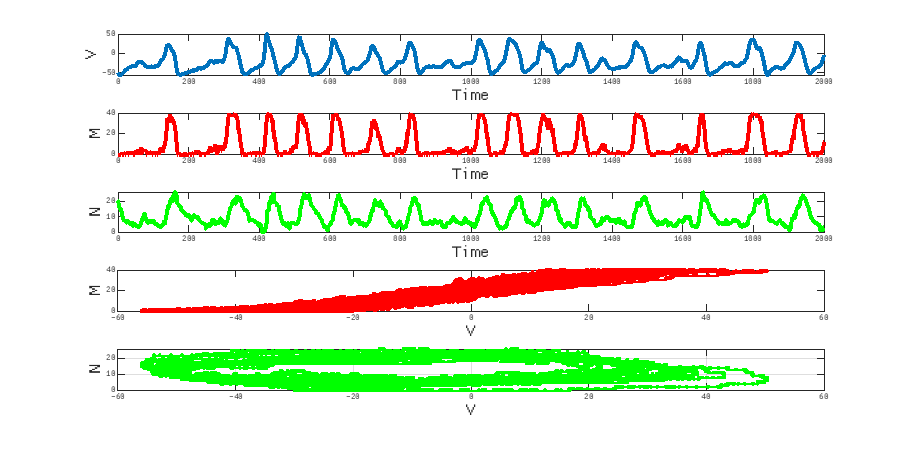
\includegraphics[width=\textwidth]{Figures/ml-gill-4}
		\caption{The Morris Lecar stochastic model with only potassium channels. From top to bottom: \textbf{1} The membrane voltage. \textbf{2} The number of open calcium channel over time. \textbf{3} The number of open potassium channels over time. \textbf{4} The number of open calcium channel over voltage. \textbf{5} The number of open potassium channel over voltage}
		\label{fig:ml-gill-4}
	\end{figure}
